\documentclass{standalone}
\usepackage{tikz}
\usetikzlibrary{patterns, positioning}


\begin{document}
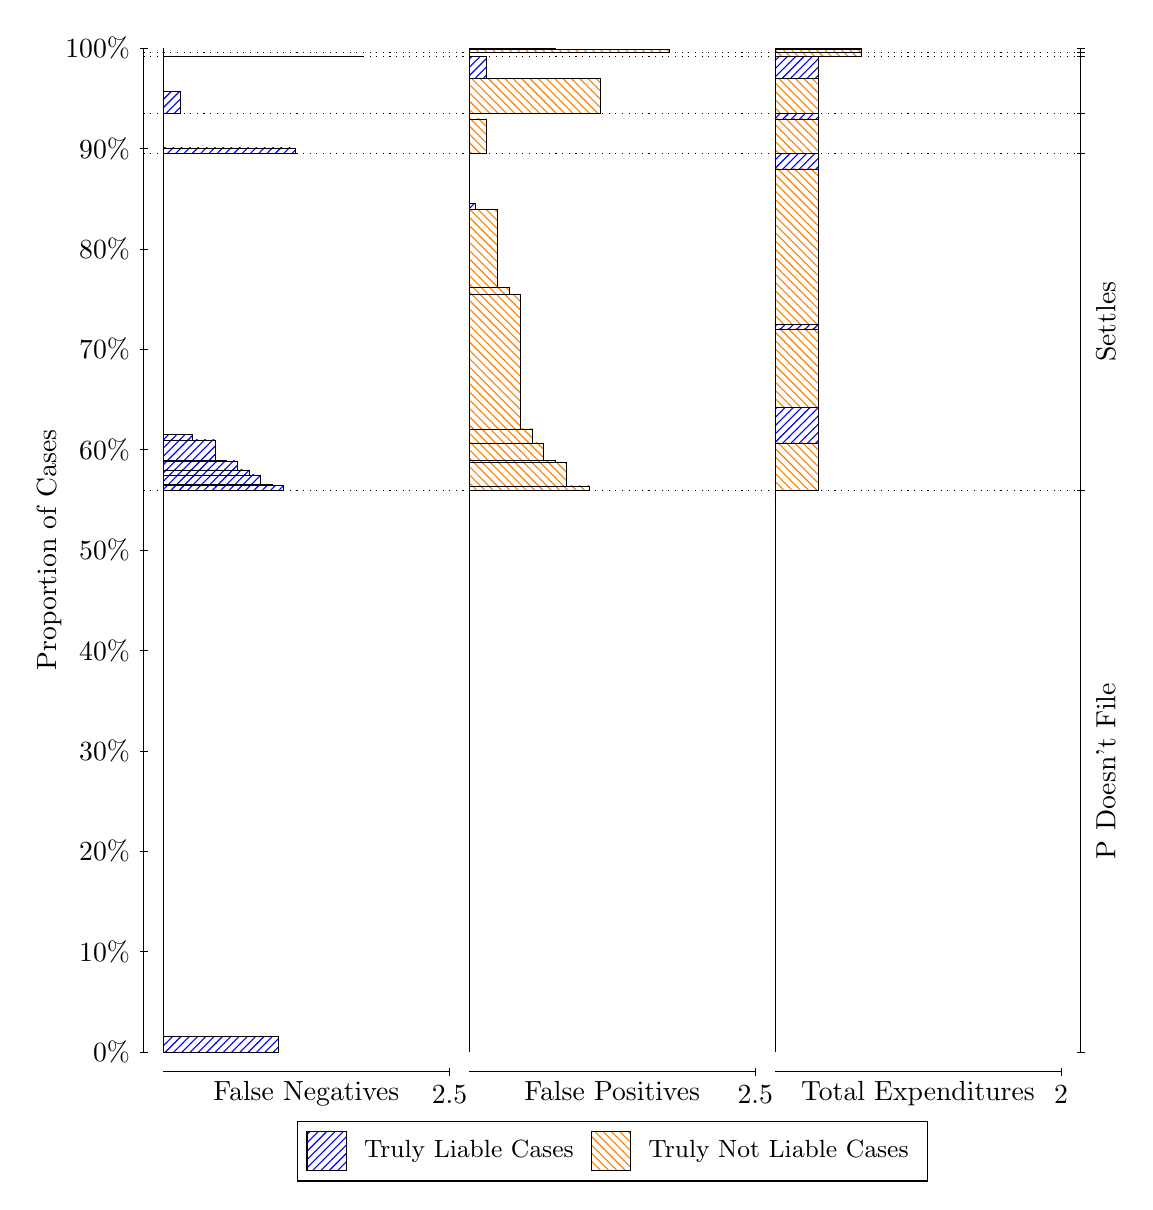
\begin{tikzpicture}
\draw[black, very thin] (1.5,1.75) -- (1.5,14.5);
\node[rotate=90, text=black, anchor=center] at (0.3, 8.125) {Proportion of Cases};
\draw[black, very thin] (1.45,1.75) -- (1.55,1.75);
\node[text=black, anchor=east] at (1.45, 1.75) {0\%};
\draw[black, very thin] (1.45,3.025) -- (1.55,3.025);
\node[text=black, anchor=east] at (1.45, 3.025) {10\%};
\draw[black, very thin] (1.45,4.3) -- (1.55,4.3);
\node[text=black, anchor=east] at (1.45, 4.3) {20\%};
\draw[black, very thin] (1.45,5.575) -- (1.55,5.575);
\node[text=black, anchor=east] at (1.45, 5.575) {30\%};
\draw[black, very thin] (1.45,6.85) -- (1.55,6.85);
\node[text=black, anchor=east] at (1.45, 6.85) {40\%};
\draw[black, very thin] (1.45,8.125) -- (1.55,8.125);
\node[text=black, anchor=east] at (1.45, 8.125) {50\%};
\draw[black, very thin] (1.45,9.4) -- (1.55,9.4);
\node[text=black, anchor=east] at (1.45, 9.4) {60\%};
\draw[black, very thin] (1.45,10.675) -- (1.55,10.675);
\node[text=black, anchor=east] at (1.45, 10.675) {70\%};
\draw[black, very thin] (1.45,11.95) -- (1.55,11.95);
\node[text=black, anchor=east] at (1.45, 11.95) {80\%};
\draw[black, very thin] (1.45,13.225) -- (1.55,13.225);
\node[text=black, anchor=east] at (1.45, 13.225) {90\%};
\draw[black, very thin] (1.45,14.5) -- (1.55,14.5);
\node[text=black, anchor=east] at (1.45, 14.5) {100\%};

\draw[black, very thin] (13.4,1.75) -- (13.4,14.5);
\draw[black, very thin] (13.35,1.75) -- (13.45,1.75);
\node[anchor=west] at (13.35, 1.75) {};
\draw[black, very thin] (13.35,8.8843) -- (13.45,8.8843);
\node[anchor=west] at (13.35, 8.8843) {};
\draw[black, very thin] (13.35,13.164) -- (13.45,13.164);
\node[anchor=west] at (13.35, 13.164) {};
\draw[black, very thin] (13.35,13.668) -- (13.45,13.668);
\node[anchor=west] at (13.35, 13.668) {};
\draw[black, very thin] (13.35,14.393) -- (13.45,14.393);
\node[anchor=west] at (13.35, 14.393) {};
\draw[black, very thin] (13.35,14.448) -- (13.45,14.448);
\node[anchor=west] at (13.35, 14.448) {};
\draw[black, very thin] (13.35,14.5) -- (13.45,14.5);
\node[anchor=west] at (13.35, 14.5) {};

\draw[black, very thin, pattern color=blue, pattern=north east lines] (1.75,1.75) rectangle (3.2033,1.9494);
\draw[black, very thin, pattern color=orange, pattern=north west lines] (1.75,1.9494) rectangle (1.75,8.8843);
\draw[black, very thin, pattern color=blue, pattern=north east lines] (1.75,8.8843) rectangle (3.276,8.9451);
\draw[black, very thin, pattern color=blue, pattern=north east lines] (1.75,8.9451) rectangle (3.1307,8.9617);
\draw[black, very thin, pattern color=blue, pattern=north east lines] (1.75,8.9617) rectangle (2.9853,9.0786);
\draw[black, very thin, pattern color=blue, pattern=north east lines] (1.75,9.0786) rectangle (2.84,9.1436);
\draw[black, very thin, pattern color=blue, pattern=north east lines] (1.75,9.1436) rectangle (2.6947,9.2556);
\draw[black, very thin, pattern color=blue, pattern=north east lines] (1.75,9.2556) rectangle (2.5493,9.2674);
\draw[black, very thin, pattern color=blue, pattern=north east lines] (1.75,9.2674) rectangle (2.404,9.5234);
\draw[black, very thin, pattern color=blue, pattern=north east lines] (1.75,9.5234) rectangle (2.1133,9.5946);
\draw[black, very thin, pattern color=orange, pattern=north west lines] (1.75,9.5946) rectangle (1.75,13.164);
\draw[black, very thin, pattern color=blue, pattern=north east lines] (1.75,13.164) rectangle (3.4213,13.231);
\draw[black, very thin, pattern color=orange, pattern=north west lines] (1.75,13.231) rectangle (1.75,13.668);
\draw[black, very thin, pattern color=blue, pattern=north east lines] (1.75,13.668) rectangle (1.968,13.949);
\draw[black, very thin, pattern color=orange, pattern=north west lines] (1.75,13.949) rectangle (1.75,14.393);
\draw[black, very thin, pattern color=blue, pattern=north east lines] (1.75,14.393) rectangle (4.2933,14.397);
\draw[black, very thin, pattern color=orange, pattern=north west lines] (1.75,14.397) rectangle (1.75,14.448);
\draw[black, very thin, pattern color=orange, pattern=north west lines] (1.75,14.448) rectangle (1.75,14.487);
\draw[black, very thin, pattern color=blue, pattern=north east lines] (1.75,14.487) rectangle (1.75,14.5);
\draw[black, very thin, pattern color=orange, pattern=north west lines] (5.6333,1.75) rectangle (5.6333,8.6849);
\draw[black, very thin, pattern color=blue, pattern=north east lines] (5.6333,8.6849) rectangle (5.6333,8.8843);
\draw[black, very thin, pattern color=orange, pattern=north west lines] (5.6333,8.8843) rectangle (7.1593,8.9388);
\draw[black, very thin, pattern color=orange, pattern=north west lines] (5.6333,8.9388) rectangle (6.8687,9.2366);
\draw[black, very thin, pattern color=orange, pattern=north west lines] (5.6333,9.2366) rectangle (6.7233,9.2634);
\draw[black, very thin, pattern color=orange, pattern=north west lines] (5.6333,9.2634) rectangle (6.578,9.4858);
\draw[black, very thin, pattern color=orange, pattern=north west lines] (5.6333,9.4858) rectangle (6.4327,9.6634);
\draw[black, very thin, pattern color=orange, pattern=north west lines] (5.6333,9.6634) rectangle (6.2873,11.368);
\draw[black, very thin, pattern color=orange, pattern=north west lines] (5.6333,11.368) rectangle (6.142,11.458);
\draw[black, very thin, pattern color=orange, pattern=north west lines] (5.6333,11.458) rectangle (5.9967,12.453);
\draw[black, very thin, pattern color=blue, pattern=north east lines] (5.6333,12.453) rectangle (5.706,12.525);
\draw[black, very thin, pattern color=blue, pattern=north east lines] (5.6333,12.525) rectangle (5.6333,13.164);
\draw[black, very thin, pattern color=orange, pattern=north west lines] (5.6333,13.164) rectangle (5.8513,13.601);
\draw[black, very thin, pattern color=blue, pattern=north east lines] (5.6333,13.601) rectangle (5.6333,13.668);
\draw[black, very thin, pattern color=orange, pattern=north west lines] (5.6333,13.668) rectangle (7.3047,14.112);
\draw[black, very thin, pattern color=blue, pattern=north east lines] (5.6333,14.112) rectangle (5.8513,14.393);
\draw[black, very thin, pattern color=orange, pattern=north west lines] (5.6333,14.393) rectangle (5.6333,14.444);
\draw[black, very thin, pattern color=blue, pattern=north east lines] (5.6333,14.444) rectangle (5.6333,14.448);
\draw[black, very thin, pattern color=orange, pattern=north west lines] (5.6333,14.448) rectangle (8.1767,14.487);
\draw[black, very thin, pattern color=blue, pattern=north east lines] (5.6333,14.487) rectangle (6.7233,14.5);
\draw[black, very thin, pattern color=orange, pattern=north west lines] (9.5167,1.75) rectangle (9.5167,8.6849);
\draw[black, very thin, pattern color=blue, pattern=north east lines] (9.5167,8.6849) rectangle (9.5167,8.8843);
\draw[black, very thin, pattern color=orange, pattern=north west lines] (9.5167,8.8843) rectangle (10.062,9.4858);
\draw[black, very thin, pattern color=blue, pattern=north east lines] (9.5167,9.4858) rectangle (10.062,9.9368);
\draw[black, very thin, pattern color=orange, pattern=north west lines] (9.5167,9.9368) rectangle (10.062,10.932);
\draw[black, very thin, pattern color=blue, pattern=north east lines] (9.5167,10.932) rectangle (10.062,10.992);
\draw[black, very thin, pattern color=orange, pattern=north west lines] (9.5167,10.992) rectangle (10.062,12.965);
\draw[black, very thin, pattern color=blue, pattern=north east lines] (9.5167,12.965) rectangle (10.062,13.164);
\draw[black, very thin, pattern color=orange, pattern=north west lines] (9.5167,13.164) rectangle (10.062,13.601);
\draw[black, very thin, pattern color=blue, pattern=north east lines] (9.5167,13.601) rectangle (10.062,13.668);
\draw[black, very thin, pattern color=orange, pattern=north west lines] (9.5167,13.668) rectangle (10.062,14.112);
\draw[black, very thin, pattern color=blue, pattern=north east lines] (9.5167,14.112) rectangle (10.062,14.393);
\draw[black, very thin, pattern color=orange, pattern=north west lines] (9.5167,14.393) rectangle (10.607,14.444);
\draw[black, very thin, pattern color=blue, pattern=north east lines] (9.5167,14.444) rectangle (10.607,14.448);
\draw[black, very thin, pattern color=orange, pattern=north west lines] (9.5167,14.448) rectangle (10.607,14.487);
\draw[black, very thin, pattern color=blue, pattern=north east lines] (9.5167,14.487) rectangle (10.607,14.5);
\draw[black, dotted] (1.5,8.8843) -- (13.4,8.8843);
\draw[black, dotted] (1.5,13.164) -- (13.4,13.164);
\draw[black, dotted] (1.5,13.668) -- (13.4,13.668);
\draw[black, dotted] (1.5,14.393) -- (13.4,14.393);
\draw[black, dotted] (1.5,14.448) -- (13.4,14.448);
\draw[black, very thin] (1.75,1.5) -- (5.3833,1.5);
\node[text=black, anchor=north] at (3.5667, 1.5) {False Negatives};
\draw[black, very thin] (5.3833,1.45) -- (5.3833,1.55);
\node[text=black, anchor=north] at (5.3833, 1.45) {2.5};

\draw[black, very thin] (5.6333,1.5) -- (9.2667,1.5);
\node[text=black, anchor=north] at (7.45, 1.5) {False Positives};
\draw[black, very thin] (9.2667,1.45) -- (9.2667,1.55);
\node[text=black, anchor=north] at (9.2667, 1.45) {2.5};

\draw[black, very thin] (9.5167,1.5) -- (13.15,1.5);
\node[text=black, anchor=north] at (11.333, 1.5) {Total Expenditures};
\draw[black, very thin] (13.15,1.45) -- (13.15,1.55);
\node[text=black, anchor=north] at (13.15, 1.45) {2};

\node[text=black, centered, rotate=90] at (13.72, 5.3172) {P Doesn't File};
\node[text=black, centered, rotate=90] at (13.72, 11.024) {Settles};





\draw (7.449999999999999,1.5) node[draw=none] (baseCoordinate) {};
\begin{scope}[align=center]
        \matrix[scale=0.5, draw=black, below=0.5cm of baseCoordinate, nodes={draw}, column sep=0.1cm]{
            \node[rectangle, draw, minimum width=0.5cm, minimum height=0.5cm, pattern color=blue, pattern=north east lines] {}; &
            \node[draw=none, font=\small, text=black] (B) {Truly Liable Cases}; &
            \node[rectangle, draw, minimum width=0.5cm, minimum height=0.5cm, pattern color=orange, pattern=north west lines] {}; &
            \node[draw=none, font=\small, text=black] (B) {Truly Not Liable Cases}; \\
            };
\end{scope}

\end{tikzpicture}
\end{document}